% Created 2021-06-22 Tue 11:30
% Intended LaTeX compiler: pdflatex
\documentclass[11pt]{article}
\usepackage[utf8]{inputenc}
\usepackage[T1]{fontenc}
\usepackage{graphicx}
\usepackage{grffile}
\usepackage{longtable}
\usepackage{wrapfig}
\usepackage[normalem]{ulem}
\usepackage{amsmath}
\usepackage{textcomp}
\usepackage{amssymb}
\usepackage{capt-of}
\usepackage{hyperref}
\usepackage[a4paper, total={6in, 8in}]{geometry}
\usepackage{amsthm}
\usepackage{amscd,mathtools,geometry,textcomp,xcolor,enumerate,titling,graphicx,subfig}
\usepackage{tikz-cd}
\usepackage{tikz}
\usepackage{svg}
\usepackage[all]{xy}
\usepackage{pgfplots}
\pgfplotsset{compat=1.15}
\usepackage{esint,mathpazo,hyperref}
\usepackage[mathletters]{ucs}
\usepackage[T1]{fontenc}
\newtheorem{theorem}{Theorem}
\newtheorem{remark}[theorem]{Remark}
\newtheorem{lemma}[theorem]{Lemma}
\newtheorem{corollary}[theorem]{Corollary}
\newtheorem{conjecture}[theorem]{Conjecture}
\newtheorem{proposition}[theorem]{Proposition}
\newtheorem{problem}{Problem}
\newtheorem{exampl}[theorem]{Example}
\newtheorem{definition}[theorem]{Definition}
\newtheorem{propdef}[theorem]{Proposition-Definition}
\newtheorem{fact}{Fact}
\newtheorem{assertion}{Assertion}
\newcommand{\re}{\mathop{\rm Re}\nolimits}
\newcommand{\im}{\mathop{\rm Im}\nolimits}
\newcommand{\coker}{\mathop{\rm coker}\nolimits}
\newcommand{\supp}{\mathop{\rm supp}\nolimits}
\newcommand{\ord}{\mathop{\rm ord}\nolimits}
\newcommand{\Spec}{\mathop{\rm Spec}\nolimits}
\newcommand{\vol}{\mathop{\rm vol}\nolimits}
\newcommand*{\transp}[2][-3mu]{\ensuremath{\mskip1mu\prescript{\smash{\mathrm t\mkern#1}}{}{\mathstrut#2}}}
\newcommand{\sff}{\mathop{\rm I\*I}\nolimits}
\newcommand{\tr}{\mathop{\rm Tr}\nolimits}
\newcommand{\const}{\mathop{\rm const }\nolimits}
\newcommand{\lcm}{\mathop{\rm lcm}\nolimits}
\newcommand{\Ric}{\mathop{\rm Ric}\nolimits}
\newcommand{\Riem}{\mathop{\rm Riem}\nolimits}
\newcommand{\Enorm}{\mathop{\mathcal{E}_{\rm norm}}\nolimits}
\newcommand{\Anorm}{\mathop{\mathcal{A}_{\rm norm}}\nolimits}
\newcommand{\Cl}{\mathop{\rm Cl }\nolimits}
\newcommand{\Spin}{\mathop{\rm Spin}\nolimits}
\newcommand{\Pin}{\mathop{\rm Pin}\nolimits}
\newcommand{\Hom}{\mathop{\rm Hom}\nolimits}
\newcommand{\End}{\mathop{\rm End}\nolimits}
\newcommand{\dive}{\mathop{\rm div}\nolimits}
\DeclareMathOperator{\hess}{Hess}
\DeclareMathOperator\arsinh{arsinh}
\newcommand\restr[2]{{% we make the whole thing an ordinary symbol
\left.\kern-\nulldelimiterspace % automatically resize the bar with \right
#1 % the function
\vphantom{\big|} % pretend it's a little taller at normal size
\right|_{#2} % this is the delimiter
}}
\author{Manh Tien NGUYEN}
\date{\today}
\title{Weighted monotonicity theorems and applications to minimal surfaces in hyperbolic space}
\hypersetup{
 pdfauthor={Manh Tien NGUYEN},
 pdftitle={Weighted monotonicity theorems and applications to minimal surfaces in hyperbolic space},
 pdfkeywords={},
 pdfsubject={},
 pdfcreator={Emacs 27.2 (Org mode 9.0.5)}, 
 pdflang={English}}
\begin{document}

\maketitle
\begin{abstract}
We show that there is a weighted version of monotonicity theorem corresponding 
to each function on a Riemannian manifold whose Hessian is a multiple of the metric tensor. 
Such function appears in the Euclidean space, the hyperbolic space \( \mathbb{H}^n \) and 
the round sphere \( \mathbb{S}^n \) as the distance function, 
the Minkowskian coordinates of \( \mathbb{R}^{n,1} \) and the Euclidean coordinates of \( \mathbb{R}^{n+1} \). 

In \( \mathbb{H}^n \), we show that the time-weighted monotonicity theorem implies the unweighted version of Anderson 
\cite{Anderson82_CompleteMinimalVarieties}. Applications include upper bounds for Graham--Witten renormalised area 
of minimal surfaces in term of the length of boundary curve and a complete computation of Alexakis--Mazzeo degrees defined in \cite{Alexakis.Mazzeo10_RenormalizedAreaProperly}. 

An argument on area-minimising cones suggests the existence of a minimal surface in \( \mathbb{H}^4 \) bounded by the Hopf
link \( \{zw=\epsilon > 0, |z|^2 +|w|^2 = 1\} \) other than the pair of disks. 
We give an explicit construction of a minimal annulus in \( \mathbb{H}^4 \) with this property and obtain by the same method
its sister in \( \mathbb{S}^4 \).

A weighted monotonicity theorem is also proved in Riemannian manifolds whose sectional curvature is bounded from above.
\end{abstract}
\section{Introduction}
\label{sec:org542a23b}

Let \(h\) be a function on a Riemannian manifold \((M,g)\) with
\(\hess h = Ug\). We will prove a monotonicity
theorem for minimal surfaces (\(k\)-dimensional orientable submanifolds with vanishing mean
curvature) in \(M\) where the area functional is weighted
by \(U\). The theorem also holds for exterior extension of a minimal surface by the
gradient flow of \(h\) in the same fashion as the extended monotonicity theorem of
Ekholm, White and Wienholtz \cite{Ekholm.etal02_EmbeddednessMinimalSurfaces}.

The existence of such function \(h\) was proved by Cheeger and Colding
\cite{Cheeger.Colding96_LowerBoundsRicci} to be equivalent to the metric locally being a warped product.
The manifold \(M\) can therefore be specialised to be the hyperbolic space \(\mathbb{H}^n\) or the round sphere \(\mathbb{S}^n\), on which the
Minkowskian coordinates \(\xi_\alpha\) and the Euclidean coordinates \(x_i\) satisfy \(\hess \xi_\alpha
  = \xi_\alpha g_{\mathbb{H}^n}\) and \(\hess x_i = -x_i g_{\mathbb{S}^n}\) respectively. 
On \(\mathbb{R}^n\), there are only 2 ways to write the
Euclidean metric locally as a warped product, either by the coordinate functions \(x_i\), in which
case the weighted monotonicity theorem trivialises, or by the distance function \(\rho
  = \sum_{i=1}^n x_i^2\) whose 
corresponding monotonicity theorem is the classical one.

In hyperbolic space, an unweighted monotonicity theorem was proved by Anderson in
\cite{Anderson82_CompleteMinimalVarieties}. We will show by a Comparison Lemma (Lemma \ref{lem:comparison}) that the
monotonicity theorem corresponding to the time coordinate implies
the unweighted version. For any surface not necessarily minimal, the Comparison Lemma
says that if its density with respect to a weight function is increasing
then so is the density with respect to any \emph{weaker}
weight. In particular, for the unit ball \(\mathbb{B}^n\) equipped
with the Poincaré, Euclidean and round-sphere metrics, one has the following chain of monotonicity
\[
   \text{time-weighted }  g_{\mathbb{H}^n} \gg   \text{unweighted } g_{\mathbb{H}^n}
   \gg g_E  \gg \text{unweighted } g_{\mathbb{S}^n}   \gg \text{weighted } g_{\mathbb{S}^n}.
  \]
A surface having increasing density with respect to an area functional in the chain
automatically has increasing density with respect to any area functional on the right of it.
This is partly the reason why our statements concerning minimal surfaces in \(\mathbb{H}^n\), which
are time-monotone, outnumber what we can say about their counterparts in \(\mathbb{S}^n\) which are at the opposite end of the chain. 

While minimal surfaces in \(\mathbb{S}^n\) are weighted-monotone, the Clifford torus of \(\mathbb{S}^3\) shows that unweighted monotonicity does not hold even in a
hemisphere. Despite this, there is a way to use Lemma \ref{lem:comparison} to obtain meaningful
statements about the unweighted area. We illustrate this by giving a geometric proof of
some results in \cite{Cheng.etal84_HeatEquationsMinimal} and
\cite{Hoffman.Spruck74_SobolevIsoperimetricInequalities}. 

One application of the monotonicity chain is the following statement about minimising cones
from \cite{Anderson82_CompleteMinimalVarieties}.

\begin{theorem}[cf. Theorem 9 of \cite{Anderson82_CompleteMinimalVarieties}]
\label{thm:minimising-cone}
If a \(k\)-dimensional radial cone \(C_\gamma\), constructed over a submanifold \(\gamma\) on the sphere at infinity of the Poincaré model is Euclidean area-minimising,
then it is the only complete minimal surface asymptotic to \(\gamma\).

In particular, area minimising cones in hyperbolic space are exactly those which are minimal in Euclidean space.
\end{theorem}

The first half of Theorem \ref{thm:minimising-cone} is slightly stronger than the second
half: Knowing that the pair of 2-planes \(zw =
0\) in \(\mathbb{C}^2\) is hyperbolic area-minimising only allows us to rule out minimal surfaces of \(\mathbb{H}^4\) 
that agree with the planes on a neighborhood of infinity.

The pair of 2-planes in \(\mathbb{R}^4\cong
\mathbb{C}^2\) that contains the Hopf link \(\{zw=\epsilon, |z|^2 + |w|^2 = 1\}\) is
not Euclidean area-minimising when \(\epsilon\in(0, \frac{1}{2})\). Theorem
\ref{thm:minimising-cone} therefore suggests another minimal
surface in the Poincaré ball filling the link. 
We will point out an explicit family of minimal annuli with this
property as the orbit of curves in the real plane \(\im z = \im w = 0\) by the quaternionic rotation \((z,w)\mapsto (ze^{i\theta},
w e^{-i\theta})\). 
The same construction also yields minimal annuli fibred by Hopf links under any metric  \(g =
e^{2\varphi(\rho)}g_E\) of \(\mathbb{R}^4\) that is conformal to the Euclidean metric by a factor \(\varphi\) depending only on \(\rho = |z|^2 +|w|^2\).

\begin{proposition}[]
\label{prop:min-annuli}
Let \(M_{C}\) be the surface in \(\mathbb{R}^4\) given by rotating the following real plane curve:
\begin{equation}
\label{eq:min-annuli}
\sin^2\psi = \frac{e^{-4\varphi}}{C^2\rho^2}, \quad C > 0
\end{equation}
where \(\psi\) is the angle formed by the tangent of the curve at a point \(p\) and the
radial direction \(\overrightarrow{Op}\). Then \(M_{C}\) is
minimal under the metric \(g =
e^{2\varphi}g_E\). Up to \(SO(4)\), the annuli \(M_{C}\) and the 2-planes are the only
minimal surfaces obtained as orbit of a real plane curve by quaternionic rotation.
\end{proposition}

In the round four-sphere, the family \(\{M_C\}\) starts with a Clifford torus and end
with a totally geodesic \(\mathbb{S}^2\). There is a countable number of parameter \(C\) in between for which the annulus \(M_C\) can be rearranged periodically to
obtain a minimally immersed torus with one-dimensional self-intersection.
The profile curves of \(M_C\) in \(\mathbb{H}^4\) and
\(\mathbb{S}^4\) are drawn in Figure \ref{fig:min-HS} for different values of \(C\). 

\begin{figure}%
    \centering
    \subfloat[\centering in \( \mathbb{H}^4 \) with \( C\) in \(\{.025, .1, .25, .5, 1, 2, 4, 8, 16, 64\} \).]{{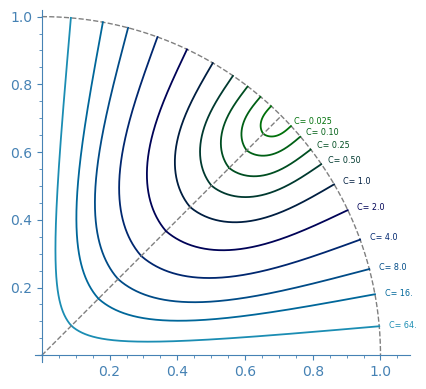
\includegraphics[width=6.5cm]{2021-01-21-minsurface-quaternion-H4.png} }}%
    \qquad
    \subfloat[\centering in \( \mathbb{S}^4 \) with \( C=6.15 \). The angle \( \theta_C\approx \frac{2\pi}{3} \). \newline The unit circle represents the Clifford torus.]{{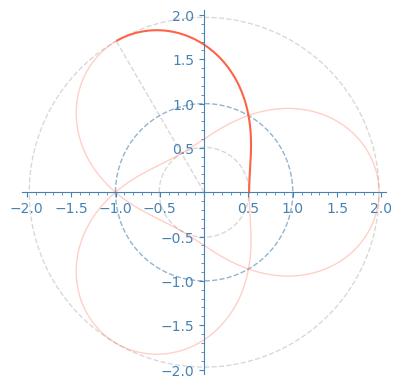
\includegraphics[width=7cm]{2021-06-3-petal.png} }}%
    \caption{The profile curve of \( M_C \)}%
    \label{fig:min-HS}%
\end{figure}

Denote by  \(\omega_{k}\) the Euclidean \(k\)-volume of \(\mathbb{S}^{k}\). Another application of monotonicity theorem is:
\begin{corollary}[]
\label{cor:intro-2pi}
The boundary at infinity of a complete \(k\)-dimensional minimal surface containing the center of
Poincaré ball has Euclidean \((k-1)\)-volume at least \(\omega_{k-1}\).
\end{corollary}

\begin{definition}
Let  \(\gamma^{k-1}\) be a submanifold of the sphere at infinity and \(p\) be an interior
point of the ball. We say that \(p\) is in the \emph{center
set} of \(\gamma\) if the Euclidean volume of \(\gamma\) in the Poincaré model centered at \(p\) is at least \(\omega_{k-1}\).
\end{definition}

Corollary \ref{cor:intro-2pi} can be rephrased as: A complete minimal surface of \(\mathbb{H}^n\) is
contained in the center set of its boundary. 
Together with the convex hull introduced in
\cite{Anderson82_CompleteMinimalVarieties}, 
the center set poses sufficient restriction on minimal surface filling a given curve to prove:

\begin{theorem}
\label{thm:separation}
Let \(L^{k-1}:=  L_1 \sqcup L_2\) be a separated union of two links \(L_1,
L_2\) in \(\mathbb{S}^{n-1}\). There is a way to rearrange \(L\) in its isotopy class such
that any minimal surface \(\Sigma^k\) in \(\mathbb{H}^n\) filling \(L\) is a disjoint union of minimal surfaces filling
each \(L_i\).
\end{theorem}
\begin{proof}
We isotope \(L\) so that \(L_1\) (respectively \(L_2\)) is contained in a small ball centered at the
North (respectively South) pole of the Poincaré ball and so that the Euclidean volume of \(L\) is less than \(\frac{1}{2}\omega_{k-1}\). 
It suffices to prove that \(\Sigma\) has no intersection with the equatorial hyperplane. By convexity, such
intersection is contained in a small ball centered at the origin \(O\). If it was
non-empty, by a small Möbius transform we could suppose that \(\Sigma\) contains \(O\) while keeping the Euclidean length of \(L\) less than \(\omega_{k-1}\). 
This contradicts Corollary \ref{cor:intro-2pi}.
\end{proof}

It was proved in \cite{Alexakis.Mazzeo10_RenormalizedAreaProperly} that:

\begin{theorem}[Alexakis--Mazzeo]
\label{thm:AM}
Let  \(\mathcal{M}_{g, b}\) be the space of properly embedded, connected \(C^{3,\alpha}\)
   two-dimensional minimal surfaces in \(\mathbb{H}^3\) of genus \(g\) and \(b\) boundary components, \(\mathcal{C}_b\)
   be the space of \(C^{3,\alpha}\) closed, embedded curves of \(b\)
   connected components in \(\mathbb{S}^2\) and  \(\Pi_{g,b}:\mathcal{M}_{g,b} \longrightarrow
   \mathcal{C}_b\) be the map which sends a surface to its boundary. Then
\begin{enumerate}
\item \(\mathcal{M}_{g, b}\) is a Banach manifold.
\item \(\Pi_{g,b}\) is proper, Fredholm, of index 0 and it has a well-defined degree \(d(g,b)\).
\end{enumerate}
\end{theorem}

Since the only minimal surface filling a round circle of
\(\mathbb{S}^2\) is a totally geodesic disk, one has \(d(0,1) = 1\) and \(d (g,1)=0\) for any \(g\geq 1\). It follows from Theorem \ref{thm:separation} that:

\begin{theorem}[]
\label{thm:AM-deg}
All Alexakis--Mazzeo degrees are zero except \(d(0,1)\).
\end{theorem}

It is of great interest to try to replace \(\mathbb{H}^3\) in the statement of Theorem \ref{thm:AM} by \(\mathbb{H}^4\). The connected components of \(\mathcal{C}_b\) would be
by definition knots (\(b=1\)) or links (\(b>1\)) and Alexakis--Mazzeo degrees would be knot/link invariants.
This direction was studied by Alves and Fine and their work will appear later. The results above
suggest that one can distinguish the Hopf link from two unlinked circles by this method. It
follows from Theorem \ref{thm:separation} that the degree among surfaces of Euler characteristic zero of the
latter vanishes while the
existence of \(M_C\) suggests that it is non-zero for the former.

The total area of a complete two-dimensional minimal surface in
\(\mathbb{H}^n\) is necessarily infinite. By looking at its expansion as
the surface runs to infinity, Graham and Witten
\cite{Graham.Witten99_ConformalAnomalySubmanifold} were able to renormalise the area to a
finite number \(\mathcal{A}_R\).
Both the time monotonicity and the space monotonicity theorems can be used to obtain upper
bounds of this number. Note that the zero set of a
space coordinate is a totally geodesic hyperplane which separates the sphere at infinity \(\mathbb{S}_\infty\) into two halves. The \emph{doubled
hyperbolic metric} is obtained by putting the \({(n-1)}\)-dimensional hyperbolic metric on 
each of them.

\begin{theorem}[]
\label{thm:upper-AR}
Let \(\Sigma^2\subset \mathbb{H}^n\) be a minimal surface with boundary \(\gamma^1\in
\mathbb{S}_\infty\). Then
\begin{equation}
\label{eq:upper-AR}
 \mathcal{A}_R(\Sigma) + \sup_{\text{round } \tilde g}|\gamma|_{\tilde g} \leq 0
\end{equation}
where the supremum is taken among metrics of curvature +1 in the standard conformal class of \(\mathbb{S}_\infty\). 
\end{theorem}

By choosing any point of \(\Sigma\) as center of the Poincaré ball and
applying Corollary \ref{cor:intro-2pi}, one has: 
\begin{corollary}[]
\label{cor:intro-AR-2pi}
\(\mathcal{A}_R(\Sigma)\leq -2\pi\) for any minimal surface \(\Sigma^2\) in \(\mathbb{H}^n\).
\end{corollary}

Corollary \ref{cor:intro-AR-2pi} can also be proved from the space version of
Theorem \ref{thm:upper-AR}.
\begin{theorem}[]
\label{thm:intro-AR-space}
If the space coordinate \(\xi_1 \geq \alpha >0\) on a minimal surface \(\Sigma^2\subset
\mathbb{H}^n\) then
   \[ 
   \mathcal{A}_R(\Sigma) + \frac{1}{2}\left(\alpha - \frac{1}{\alpha}\right)|\gamma_\infty|_{\tilde g} \leq 0  
   \]
where \(\tilde g\) is the doubled hyperbolic metric associated to \(\xi_1\).
\end{theorem}

During the preparation of this paper, Theorem \ref{thm:upper-AR} and Corollary \ref{cor:intro-AR-2pi} were independently proved by Bernstein 
in \cite{Bernstein21_SharpIsoperimetricProperty} using the work of Choe and Gulliver
\cite{Choe.Gulliver92_SharpIsoperimetricInequality}. It was via
\cite{Bernstein21_SharpIsoperimetricProperty} that the author learned about
\cite{Choe.Gulliver92_SharpIsoperimetricInequality} and its companion
\cite{Choe.Gulliver92_IsoperimetricInequalitiesMinimal}. Theorem \ref{thm:monotonicity-H-time} and
\ref{thm:monotonicity-S} are indeed Theorem 3 of \cite{Choe.Gulliver92_IsoperimetricInequalitiesMinimal}, the time-weighted area in \(\mathbb{H}^n\) and the weighted area in \(\mathbb{S}^n\) (Section 3) were called
\emph{modified volume} there. The fact that a minimal surface in \(\mathbb{H}^n\) has less
area than the cone built upon its boundary (Proposition 2 of
\cite{Choe.Gulliver92_SharpIsoperimetricInequality}, Corollary \ref{cor:2pi} in this text) was crucial to the proof of sharp
isoperimetric inequality \(4\pi A + A^2 \leq L^2\), where \(A\) is the area of a two-dimensional minimal surface
and \(L\) is the length of its boundary. By this fact, since
\(4\pi A + A^2\) is increasing in \(A\), it suffices to check the inequality only for
cones. The Comparison Lemma \ref{lem:comparison} allows us to arrive at Corollary \ref{cor:2pi} in a 
simpler way than \cite{Choe.Gulliver92_SharpIsoperimetricInequality}.


One can hope, since a monotonicity theorem is an inequality, that the results above still
 hold when the Hessian of the function \(h\) is comparable to the metric as symmetric
 2-tensors. Such function arises naturally as the distance function in a Riemannian
 manifold whose sectional curvature is bounded from above. We explore this
 idea in Section 5. We note that although the unweighted monotonicity theorem does
 not hold in case of positive curvature, an unweighted monotonicity \emph{inequality} was obtained
 by Scharrer \cite{Scharrer21_GeometricInequalitiesVarifolds}.

\paragraph{Acknowledgements.}
The author thanks Joel Fine for introducing him to minimal surfaces and
harmonic maps in hyperbolic space, for proposing the search of the minimal annuli \(M_C\) and
for other valuable discussions. The paper
\cite{Hoffman.Spruck74_SobolevIsoperimetricInequalities} was pointed out to him by Christian Scharrer. The author was supported by 
\emph{Excellence of Science grant number 30950721, Symplectic techniques in differential geometry}.

\section{The hyperbolic space and the sphere as warped spaces.}
\label{sec:orga423e7a}
A metric on a Riemannian manifold \(M=N\times [a,b]\) is a \emph{warped product} if it has the
 form 
\begin{equation}
\label{eq:warped-metric}
 g = dr^2 + f^2(r) g_N 
\end{equation}
where \(r\in [a,b]\) and \(g_N\) is a Riemannian metric on \(N\). It can be checked that an anti-derivative \(h\) of the warping function \(f\) satisifies  \(\hess(h) =
f'(r) g\). On the other hand, if such function \(h\) exists, the space is locally
warped by its level sets \cite{Cheeger.Colding96_LowerBoundsRicci}.

\begin{proposition}[cf. \cite{Cheeger.Colding96_LowerBoundsRicci}]
\label{prop:cheeger-colding}
Suppose that there exists a function \(h\) on \((M,g)\) with no critical point,
whose level set are connected and 
\begin{equation}
\label{eq:xi}
\hess h = U.g
\end{equation}
for a function \(U\in C^0(M)\). Then:
\begin{enumerate}
\item \(U=U(h)\) is a function of \(h\), i.e. a composition of \(h\) and a function \(U:
   \mathbb{R}\longrightarrow \mathbb{R}\). The function \(V:= |dh|^2\in C^1(M)\) is
also a function of \(h\) and one has \(U = \frac{1}{2}V'\).
\item The metrics \(g_a, g_b\) induced from \(g\) on level sets \(h^{-1}(a)\) and \(h^{-1}(b)\) are related
by \(\frac{g_a}{V(a)}= \frac{g_b}{V(b)}\) via the inverse gradient flow of \(h\). 
This defines a metric \(\tilde g\) on level sets under which the flow is isometric. 
The metric \(g\) on \(M\) pulls back
via the flow map \(h^{-1}(a)\times {\rm Range}(h) \longrightarrow M\) to
\[
    g = \frac{V(h)}{V(a)}g_a + \frac{dh^2}{V(h)} = V(h)\tilde g + \frac{dh^2}{V(h)},
   \]
which is a warped product after a change of variable \(dr = \frac{dh}{V(h)^{1/2}}\).
\end{enumerate}
\end{proposition}

\begin{proof}
For any vector field \(v\), one has 
\[
 v(V) = 2 g(\nabla_v \nabla h, \nabla h)= 2 \hess(h)(v, \nabla h) = 2U g(v, \nabla h)
\]
It follows, by first taking \(v\) to be any vector field tangent to level
sets of \(h\), then to be the inverse gradient \(u:= \frac{\nabla h}{|\nabla h|^2}\), that
\(V\) is constant on the level sets, and as a function of \(h\), \(V' = 2U\).

For the second part, let \(v_t\) be a vector field of \(M\) tangent to level sets \(h^{-1}(t)\) given by 
pushing forward via the flow of \(u\) a vector field \(v_a\) tangent to \(h^{-1}(a)\). The Lie bracket \([v_t, u]\)
vanishes by definition and for all time \(t\),
\[
 \frac{d}{dt}|v_t|^2 = 2 g(\nabla_u v_t, v_t) = 2 g(\nabla_{v_t}u, v_t) =
\frac{2}{|\nabla h|^2}\hess(h)(v_t, v_t) = \frac{V'}{V}|v_t|^2.
\]
This means that \(\frac{|v_t|^2}{V(t)}\) is constant along the flow and so \(\frac{g_a}{V(a)} = \frac{g_b}{V(b)}\) for all \(a,b\in {\rm Range}(h)\).
\end{proof}

We note that \(\tilde g\) is the metric \(g_N\) in \eqref{eq:warped-metric}. We will use
\(\tilde g\) to denote the metric \(V(h)^{-1}g\) on \(M\). 

In applications, we will only assume that the function \(h\) satisfies
\eqref{eq:xi} on \(M\) and it can have critical points, as in the following examples.

\begin{exampl}[]
\label{ex:xi-R}
In Euclidean space \(\mathbb{R}^n\), the only functions satisfying
   \eqref{eq:xi} are the coordinates \(x_i, i=1,\dots,n\) with \(U=0, V=1\) and the square of distance \(\rho := \frac{1}{2}\sum_{i=1}^n
   x_i^2\) with \(U= 1, V = 2\rho\).
\end{exampl}

\begin{exampl}[]
\label{ex:xi-S}
In the unit sphere \(\mathbb{S}^n = \{(x_1,\dots, x_n, x_{n+1})\in
\mathbb{R}^{n+1}:\sum_{i=1}^{n+1} x_i^2 = 1\}\), the Euclidean coordinates \(x_i\)
 satisfy \eqref{eq:xi} with \(U = -x_i, V = 1-x_i^2\). 
\end{exampl}

\begin{exampl}[]
\label{ex:xi-H}
In the hyperbolic space \(\mathbb{H}^n=\{(\xi_0,\dots,\xi_n)\in \mathbb{R}^{n,1}:
   \xi_0^2 - \sum_{i=1}^n\xi_i^2=1, \xi_0 > 0\}\), the Minkowskian coordinates \(\xi_\alpha\) satisfies
   \eqref{eq:xi} with \(U=\xi_\alpha, V = \xi_\alpha^2 + |\partial_{\xi_\alpha}|^2\),
   where  \(|\partial_{\xi_\alpha}|^2\) is the Minkowskian norm, which is -1 for
   time-like unit
   vectors and +1 for space-like ones.

Unlike the round sphere, the hyperbolic space can be written as a warped
product in two different ways up to isometry. Each interior point corresponds to a
unique time coordinate \(\xi_0\) that it minimises and 
each oriented totally geodesic hyperplane
corresponds to a unique space coordinate \(\xi_1\) that
vanishes on it. Note that no other level set of \(\xi_1\) is totally
geodesic.
\end{exampl}

We remark that metric \(\tilde g\) in the case \((\mathbb{R}^n, \rho), (\mathbb{S}^n, x_i)\) and
   \((\mathbb{H}^n, \xi_0)\) is the round metric on \(\mathbb{S}^{n-1}\). For \((\mathbb{H}^n, \xi_1)\), \(\tilde g\)
   is the doubled hyperbolic metric on \(\mathbb{S}^{n-1}\). 

\section{Monotonicity Theorems and Comparison Lemma}
\label{sec:orga12f250}

The following lemma often appears as \(\dive_\Sigma X^\Sigma = \dive_\Sigma X + k(\Sigma)X\) where \(\Sigma\) is a submanifold of \(M\), \(X\) is a vector
field along \(\Sigma\) and \(X^\Sigma\) is its tangent component to \(\Sigma\). Similarly, we will denote the gradient vector in \(M\) of a function \(h\) by \(\nabla
h\) and its projection to \(\Sigma\) by \(\nabla^\Sigma h\).
\begin{lemma}[Leibniz rule]
\label{lem:chain-rule}
Let \(f:(\Sigma^k,g_\Sigma) \longrightarrow (M^n, g)\) be a map between Riemannian manifolds and \(\tau(f)\) be its tension
field, then for any \(C^2\) function \(h\) on \(M\), one has
\begin{equation}
\label{eq:chain-rule}
\Delta_{\Sigma} (h\circ f) = \tr_{\Sigma} f^*\hess h + dh.\tau(f)
\end{equation}
In particular, the Laplacian of \(h\) on a submanifold \(\Sigma\) is given by 
\begin{equation}
\label{eq:hess-lap}
\Delta_\Sigma h = \tr_\Sigma \hess h  
\end{equation} 
if \(\Sigma\) is either minimal or tangent to the gradient of \(h\) at the point in question.
\end{lemma}

\subsection{Weighted monotonicity}
\label{sec:org98d5763}

Condition \eqref{eq:xi} forces all non-degenerate critical points of \(h\) to be either
 local maxima or local minima. The functions in Examples \ref{ex:xi-R},
\ref{ex:xi-S}, \ref{ex:xi-H} fall into two types:
\begin{enumerate}
\item \(h\) has no other critical value than its minimum \(h_{\min}\) and the sublevel sets
\(\{h\leq t\}\) are compact. 
This is the case of \((\mathbb{R}^n,\rho), (\mathbb{S}^n\setminus\{\rm pt\},x_i)\) and \((\mathbb{H}^n,\xi_0)\).
\item \(h\) has no critical point and the sublevel sets are no longer
compact, as in the case of \((\mathbb{H}^n,\xi_1)\).
\end{enumerate}

Given a subset \(\gamma\) of a level set of \(h\), the \emph{\(h\)-tube} \(T_{\gamma}(t_1, t_2)\) is obtained by flowing \(\gamma\) along the
gradient field of \(h\) from level \(h=t_1\) to level \(h=t_2\). When \(h\) is of the first type and \(t_1=h_{\min}\), this is visually a cone.

For a function \(h\) of the first type, we define the \emph{weighted area} and the \emph{weighted density} of a surface \(\Sigma^k\) to be
\begin{equation}
\label{eq:xi-weighted-area}
 A_h(\Sigma)(t) := \int_{\Sigma,h\leq t}U,\qquad \Theta^A_h(t) := \frac{A_h(t)}{\frac{\omega_{k-1}}{k}V^{k/2}(t)}.
\end{equation}
Note that the denominator of \(\Theta_h^A\) is up to constant the weighted area of
a tube \(T_\gamma(h_{\min},t)\):
\begin{equation}
\label{eq:area-tube-1}
A_h(T_\gamma)= \frac{|\gamma|}{k} \left(V(t)^{k/2}- V(h_{\min})^{k/2}\right) = \frac{|\gamma|}{k} V(t)^{k/2}
\end{equation}
where \(|\gamma|\) is the volume of \(\gamma\) under the metric \(\tilde g\).

For the second type, it is possible that the integral
in \eqref{eq:xi-weighted-area} does not converge. One can remedy this by only counting
area in the region \(h\geq h_0\). We will assume that \(\Sigma\) intersects
the level set \(h^{-1}(h_0)\) at a smooth \((k-1)\)-dimensional submanifold \(\gamma_0\) and define the weighted area and the weighted density by
\begin{equation}
\label{eq:xi-weighted-area-plus}
B_h(\Sigma)(t):= \int_{\Sigma,h_0\leq h\leq t}U(h) + \frac{1}{k}\int_{\gamma_0}|\nabla^\Sigma h|,\qquad \Theta_h^B:=
\frac{B_h(t)}{\frac{\omega_{k-1}}{k}V^{k/2}(t)}.
\end{equation}
which are finite for a large class of surfaces. The denominator of \(\Theta^B_h\) is again the
weighted area of a tube \(T_\gamma(h_0,t)\):
\begin{equation}
\label{eq:area-tube-2}
 B_h(T_\gamma)= \frac{|\gamma|}{k}(V(t)^{k/2} - V(h_0)^{k/2}) + \frac{|\gamma|}{k}V(h_0)^{k/2} = \frac{|\gamma|}{k}V(t)^{k/2}.
\end{equation}

\begin{theorem}[Weighted Monotonicity]
\label{thm:monotonicity-warped}
Suppose that \(h\) is a \(C^2\) function on a Riemannian manifold \(M\) that
satisfies \eqref{eq:xi} with \(U\) and \(V= |\nabla h|^2\) being functions of \(h\)
such that \(U = \frac{1}{2}V'\). Let \(\Sigma^k\) be a minimal
surface in \(M\).
Assume that the integral in \eqref{eq:xi-weighted-area} (respectively
\eqref{eq:xi-weighted-area-plus})  is finite, then \(\frac{d}{dt}\Theta^A_h\)
(respectively \(\frac{d}{dt}\Theta^B_h\) ) has the same sign as \(U\).

Moreover, the conlusion still holds for an extension  \(\tilde\Sigma\)  of a minimal
surface \(\Sigma^k\subset\{h \leq t_0\}\) whose boundary \(\gamma^{k-1}\) is piecewise
smooth and contained in \(h^{-1}(t_0)\) by an 
exterior \(h\)-tube \(T_{\gamma}(t_0, t)\) built upon \(\gamma\). 

In both case,  \(\frac{d}{dt}\Theta^A_h\) (respectively \(\frac{d}{dt}\Theta^B_h\) )
vanishes if and only if the gradient of \(h\) is tangent to \(\Sigma\).
\end{theorem}
\begin{proof}
It follows from Lemma \ref{lem:chain-rule} that \(\Delta_\Sigma h = kU\) on \(\Sigma\). By
Stokes' theorem,
\begin{equation}
\label{eq:stokes}
A_h(t) = \int_{\Sigma,h\leq t} U(h) = \frac{1}{k}\int_{\Sigma,h\leq t}\Delta_\Sigma h = \frac{1}{k}\int_{\Sigma,h=t}\nabla^\Sigma h\cdot n = \frac{1}{k}\int_{\Sigma,h=t}|\nabla^\Sigma h|
\end{equation}
because the outer normal of \(\{h\leq t\}\) in \(\Sigma\) is \(n=
\frac{\nabla^{\Sigma} h}{|\nabla^{\Sigma} h|}\). By the coarea formula, 
\[
 \frac{dA_h}{dt} = U(t)\int_{\Sigma,h = t} \frac{1}{|\nabla^\Sigma h|}.
\]
Combining this with \eqref{eq:stokes} and \(|\nabla^\Sigma h|^2\leq  V(h)\), one has \(\frac{1}{U}\frac{dA_h}{dt} \geq \frac{k A}{V}\), or
\(\frac{1}{U} \frac{d}{dt}(\frac{A_h}{V^{k/2}})\geq 0\).

Similarly, one has \(B_h(t) = \frac{1}{k}\int_{\Sigma,h = t}|\nabla^\Sigma h|\), and
\(\frac{dB_h}{dt} = U(t)\int_{\Sigma,h = t} \frac{1}{|\nabla^\Sigma h|}\) and the
same conclusion is drawn for the second type function.

For cone extension, it suffices to rewrite equation \eqref{eq:stokes} when \(t > t_0\) as
   \[
    kA_h(t) = \left(\int_{\Sigma,h\leq t_0}+
   \int_{T_{\gamma}(t_0,t)}\right)\Delta h =
   \int_{\tilde\Sigma,h=t}|\nabla^{\tilde\Sigma} h| +
   \int_{\gamma}\left( |\nabla^\Sigma h| - |\nabla^M h|  \right)\leq
   \int_{\tilde\Sigma,h=t}|\nabla^{\tilde\Sigma} h|.
   \]
\end{proof}

\begin{remark}
\label{rem:monotonicity-warped}
\begin{enumerate}
\item If \(\Sigma\) contains a multiple of \(\gamma\), the area of the tube should be counted with multiplicity.
\item We only need the "\(\leq\)" sign in \eqref{eq:stokes} and hence it suffices that \(\Delta_\Sigma h \geq k U(h)\). Theorem \ref{thm:monotonicity-warped}
still holds if \(\hess h\geq
   U.g\), provided that \(U\) and \(V = |d h|^2\) are still
functions of \(h\) and that \(U = \frac{1}{2}V'\).
\end{enumerate}
\end{remark}

\begin{remark}
\label{rem:monotonicity-current}
When \(\Sigma\) is a stationary rectifiable \(k\)-current, the proof of Theorem
   \ref{thm:monotonicity-warped} can be adapted in the same fashion as
   \cite{Anderson82_CompleteMinimalVarieties} and  \cite{Ekholm.etal02_EmbeddednessMinimalSurfaces}. We replace the integration by part \eqref{eq:stokes}
   by the first variation formula of current, which reads \(\int_\Sigma
   {\rm div}_\Sigma X\ d\|\Sigma\| = 0\) where \(X\) is any smooth vector field and
   \(d\|\Sigma\|\) is the mass measure. We recover \(k A_h - \frac{V}{U}A'_h \leq 0\)
   by choosing  \(X:= \chi(h)\nabla h\) where \(\chi\) is a decreasing function that approximates the characteristic
   function of \([-\infty, t]\), and by noting that \(\dive_\Sigma X =   \chi' |\nabla^\Sigma h|^2 + \chi\Delta_\Sigma h \geq \chi' V + k \chi U\).

For the tube extension and the formulation of \(B_h\) when \(h\) is of the second
   type, we replace the intersection \(\gamma =\Sigma \cap h^{-1}(t_0)\) (or \(\gamma_{0} = \Sigma\cap h^{-1}(h_0)\) respectively) by an
   \(\mathcal{H}^{k-1}\)-rectifiable set such that the pair  \((\Sigma, \gamma)\) is \emph{strongly stationary}. This means that 
\(\int_\Sigma {\rm div}_\Sigma X
   \leq \int_{\gamma} |X^\perp|\) 
for any smooth vector field \(X\) whose normal
   component to \(\gamma\) is \(X^\perp\), or equivalently that there exists an \(\mathcal{H}^{k-1}\)-measurable normal vector field \(\nu\) on \(\gamma\) with \(\sup|\nu| \leq 1\) such that \(\int_\Sigma {\rm div}_\Sigma X = \int_\gamma g(X,\nu)\). 
The definition \eqref{eq:xi-weighted-area-plus} should be rewritten for strongly stationary
   pair \((\Sigma,\gamma_0)\) as
\[ B_h(\Sigma)(t):= \int_{\Sigma}U(h) - \frac{1}{k}\int_{\gamma_0}g(\nabla h,\nu_0).
\]
\end{remark}
Theorem \ref{thm:monotonicity-warped} can also be extended for harmonic maps. Given a map \(f:\Sigma \longrightarrow M\), we
define its \emph{dimension at a point} \(p\in \Sigma\) to be the ratio \(\frac{|df_p|^2}{|df_p|_o^2}\)
of the tensor norm of the derivative at \(p\) (called energy
density) and its operator norm, or \(+\infty\) if the latter vanishes. Note that when \(df_p\) is non-zero and conformal, 
this is the dimension of \(\Sigma\). The \emph{dimension} of \(f\), defined as the smallest
dimension among all points, will play the role of \(k\) in our argument.

The \emph{weighted Dirichlet energy} of \(f\)
in the region \(h\leq t\) is defined as \(E_h(t):=\int_{\Sigma, h\circ f\leq t} U |df|^2\) or \(E_h(t):=
\int_{\Sigma, h_0\leq h\circ f\leq t} U|df|^2 + \int_{\Sigma,h\circ f = h_0}|d(h\circ f)|\)
depending on the type of \(h\). The \emph{weighted density} is \(\Theta_h(t):= \frac{E_h(t)}{V(t)^{k/2}}\).

\begin{theorem}
\label{thm:monotonicity-map}
Let \(h, U, V\) be as in Theorem \ref{thm:monotonicity-warped} and
\(f:\Sigma \longrightarrow M\) be a harmonic map. Then \(\frac{d}{dt}\Theta_h\) has the same sign as \(U\). 
\end{theorem}
\begin{proof}
By Lemma \ref{lem:chain-rule} one has \(\Delta (h\circ f) = U |df|^2\) and by
integration by part, \(E_h(t) = \int_{\Sigma, h\circ f = t} |d(h\circ f)|\). One then
compares \(E_h\) with its derivative obtained from coarea formula \(\frac{dE_h}{dt} = U(t) \int_{\Sigma, h\circ f = t}
\frac{|df|^2}{|d(h\circ f)|}\).
The definition of 
\(k\) guarantees \(\frac{|df|^2}{|d(h\circ f)|} \geq k \frac{|d(h\circ f)|}{|dh|^2}\) and therefore \(U^{-1}\frac{dE_h(t)}{dt} \geq \frac{k}{V}E_h\). 
\end{proof}


We will restate Theorem \ref{thm:monotonicity-warped} when \(M\) is the hyperbolic space
and the sphere. 

Given a time coordinate \(\xi_0\) of \(\mathbb{H}^n\),
the \emph{time-weighted area} functional is defined as
\[
 A_{\xi_0}(\Sigma)(t):= \int_{\Sigma,1\leq \xi_0\leq t}\xi_0,
\]
For a totally geodesic copy of \(\mathbb{H}^k\) in \(\mathbb{H}^n\) passing by \(\xi_0^{-1}(1)\), it is given by
\(A_{\xi_0}(\mathbb{H}^k)(t)={\frac{\omega_{k-1}}{k}(t^2-1)^{k/2}}\).
Define the \emph{time-weighted density} by \(\Theta_{\xi_0}(\Sigma)(t):=\frac{A_{\xi_0}(\Sigma)(t)}{A_{\xi_0}(\mathbb{H}^k)(t)}\) and substitute \(h=\xi_0\) into Theorem
\ref{thm:monotonicity-warped}, one has:
\begin{theorem}[Time Monotonicity]
\label{thm:monotonicity-H-time}
The time-weighted density of an extension by exterior
\(\xi_0\)-tube of a minimal
surface is increasing on \((1,+\infty)\).
\end{theorem}

To state the weighted monotonicity theorem corresponding to a space coordinate \(\xi_1\),
we will assume that the surface \(\Sigma^k\) is contained in the region \(\{\xi_1 \geq 0\}\) and that its boundary consists of a (possibly empty) part
\(\gamma_0\) in \(\xi_1^{-1}(0)\) and a part \(\gamma_\infty\) in \(\mathbb{S}_\infty\), both of them
are disjoint from the equator \(\xi_1^{-1}(0) \cap \mathbb{S}_{\infty}\).
The \emph{space-weighted area} functional is defined by
\[
B_{\xi_1}(\Sigma)(t):=\int_{\Sigma, 0\leq\xi_1\leq t}\xi_1 + \frac{1}{k}\int_{\Sigma,\xi_1=0}|\nabla^\Sigma\xi_1|
\]
and is finite for such surface \(\Sigma\). In particular, if  \(\gamma^{k-1}\) is a submanifold in the interior of \(\xi_1^{-1}(0)\) with hyperbolic volume \(|\gamma|\), the \(\xi_1\)-tube  \(T_\gamma(0,t)\) built upon \(\gamma\) has space-weighted area \(\frac{|\gamma|}{k}(t^2+1)^{k/2}\).
The \emph{space-weighted density} is defined as \(\Theta_{\xi_1}(t):=\frac{B_{\xi_1}(\Sigma)(t)}{\frac{\omega_{k-1}}{k}(t^2+1)^{k/2}}\) and is
constant for such tube.
\begin{theorem}[Space Monotonicity]
\label{thm:monotonicity-H-space}
The space-weighted density of an extension by exterior \(\xi_1\)-tube of a minimal
surface is increasing on \((0,+\infty)\).
\end{theorem}

When \(M\) is the round sphere \(\mathbb{S}^n\) seen as a warped space using an Euclidean coordinate \(x=x_i\), we
define the \emph{weighted area} and \emph{weighted density} by
\[
 A_x(\Sigma)(t):= \int_{\Sigma,x\geq t}x,\qquad \Theta_x(\Sigma)(t) :=
\frac{A_x(\Sigma)(t)}{A_x(\mathbb{S}^k)(t)}.
\]
A totally geodesic \(\mathbb{S}^k\subset \mathbb{S}^n\) passing by \(x^{-1}(1)\) has  \(A_x(\mathbb{S}^k)(t) = \frac{\omega_{k-1}}{k}(1-t^2)^{k/2}\). 
It follows from Theorem \ref{thm:monotonicity-warped} for \(h=1-x\) that:

\begin{theorem}[Weighted monotonicity in \( \mathbb{S}^n \)]
\label{thm:monotonicity-S}
The weighted density of an extension by exterior
\(x\)-tube of a minimal surface in \(\mathbb{S}^n\), is decreasing on \((0, 1)\) and increasing on \((-1,0)\).
\end{theorem}
\subsection{Comparison lemma}
\label{sec:org2a3cdb8}

It is useful to weight the area functional of \eqref{eq:xi-weighted-area} by a
function \(P(h)\) other than \(U(h)\). The \emph{\(P\)-area} is defined
by 
\[ 
A_P(\Sigma)(t):= \int_{\Sigma,h\leq t}P(h), \quad B_P(\Sigma)(t):=\int_{\Sigma,h_0\leq h\leq t}P(h) +
\frac{1}{k}\int_{h=h_0}|\nabla^\Sigma h|.
\]
We normalise
the \(P\)-area of a minimal surface by that of an \(h\)-tube,
which is up to a factor
\begin{equation}
\label{eq:Q}
Q(t):=
\begin{cases}
\omega_{k-1}\int_{h\leq t} P(h)V^{\frac{k}{2}-1}(h) dh,  & \text{if $h$ is of the first type}, \\
\omega_{k-1}\left(\int_{h=h_0}^t P(h)V^{\frac{k}{2}-1}(h)dh + \frac{1}{k}V(h_0)^{k/2}\right) & \text{if $h$ is of the second type}
\end{cases}
\end{equation}
and define the \emph{\(P\)-density} as 
\(\Theta_P(\Sigma)(t):= \frac{A_P(t)}{Q(t)}\) or \(\frac{B_P(t)}{Q(t)}\)
respectively. When \(P=U\), these are the weighted area/density defined in
\eqref{eq:xi-weighted-area} and \eqref{eq:xi-weighted-area-plus}. We will always assume that the weight function is positive in the relevant
region of \(M\). 
\begin{exampl}[]
\label{ex:weight-P}
\begin{enumerate}
\item On the round sphere \(\mathbb{S}^n\), modeled as the compactification of \(\mathbb{R}^n\)
with \(g_{\mathbb{S}^n}= \frac{4}{(1+r^2)^2}g_E\), the function \(x:=
   \frac{1-r^2}{1+r^2}\) is the Euclidean
coordinate of Example \ref{ex:xi-S} that is maximised at the origin and minimised at 
infinity. The Euclidean area of \(\mathbb{R}^n\) is a \(P\)-area with \(P = (1+x)^{-k}\).
\item In the Poincaré ball \(\mathbb{B}^n\) with metric \(g_{\mathbb{H}^n}=
   \frac{4}{(1-r^2)^2}g_E\), the function \(\xi_0 := \frac{1+r^2}{1-r^2}\) is the time
coordinate minimised at the center. The Euclidean area corresponds to \(P = (1+\xi_0)^{-k}\). 
The unweighted area of the round metric \(g_{\mathbb{S}^n}\) corresponds to \(P=\xi_0^{-k}\) and the \(x\)-weighted area above
corresponds to \(P = \xi_0^{-k-1}\).
\end{enumerate}
\end{exampl}

\begin{definition}
Given 2 weight functions \(P_1, P_2\) whose tube area \(Q_1, Q_2\) are defined by
\eqref{eq:Q}, we say that \(P_1\) is \emph{weaker} than \(P_2\) if \(\frac{P_1}{Q_1}\leq \frac{P_2}{Q_2}\), in other words if \(\frac{d}{dt}\frac{Q_1}{Q_2}\leq 0\), i.e. the \(P_2\)-area 
of a \(k\)-dimensional tube increases faster than its \(P_1\)-area. This is obviously
a transitive relation.
\end{definition}


\begin{lemma}[Comparison]
\label{lem:comparison}
Let \(\Sigma^k\subset M^n\) be any surface (not necessarily minimal), \(P_1, P_2\) be
two non-negative continuous
weights and \(\Theta_1,\Theta_2\) be the corresponding densities.

\begin{enumerate}
\item Suppose that \(P_1\) is weaker than \(P_2\) and that \(\frac{d\Theta_2}{dt}\geq 0\), then one has \(\Theta_1\leq\Theta_2\) and 
\[ 
   \frac{d\Theta_1}{dt} \geq \frac{Q_2}{P_2}\frac{P_1}{Q_1}
   \frac{d\Theta_2}{dt}.
   \]
In particular, the density \(\Theta_1\) is also increasing.
\item On the other hand, if \(P_2\) is weaker than \(P_1\) and \(\frac{d\Theta_2}{dt}\geq 0\), then one has \(\Theta_1\geq\Theta_2\).
\end{enumerate}
\end{lemma}
\begin{proof}
One has \(P_1^{-1} \frac{dA_{P_1}}{dt} = P_2^{-1}\frac{dA_{P_2}}{dt}\) from coarea
formula, therefore
\begin{equation}
\label{eq:comparison-1}
\frac{Q_1}{P_1}\frac{d\Theta_1}{dt} + \omega_{k-1}V^{\frac{k}{2}-1}\Theta_1 = \frac{Q_2}{P_2}\frac{d\Theta_2}{dt} + \omega_{k-1}V^{\frac{k}{2}-1}\Theta_2
\end{equation}
which can be rearranged into
\begin{equation}
\label{eq:comparison-2}
P_1^{-1} \frac{d}{dt}\left( Q_1(\Theta_1 -\Theta_2) \right) = \left(\frac{Q_2}{P_2}-\frac{Q_1}{P_1}\right) \frac{d\Theta_2}{dt}
\end{equation}
For the second part of the Lemma, it follows from the hypothesis  that the RHS of
\eqref{eq:comparison-2} is positive, and therefore \(Q_1(
\Theta_1- \Theta_2)\) is an increasing function. The latter vanishing at \(t=0\) for both types of function \(h\) means that \(\Theta_1\geq\Theta_2\)
for all time.

For the first part, the RHS of \eqref{eq:comparison-2} is negative by hypothesis and
 therefore \(\Theta_2 \geq \Theta_1\). The rest of the conclusion follows by substituing this into \eqref{eq:comparison-1}.
\end{proof}


\begin{remark}
\label{rem:comparison}
In the Poincaré ball \(\mathbb{B}^n\) (see Example \ref{ex:weight-P}), let 
   \(P_1 = \xi_0^{-k-1}\), \(P_2 =\xi_0^{-k}\), \(P_3 = (1+\xi_0)^{-k}\), \(P_4=1\) and \(P_5=\xi_0\). It can be checked that \(P_i\) is weaker than \(P_{i+1}\). Lemma
   \ref{lem:comparison} says that there is the following chain of monotonicity:
\begin{equation}
\label{eq:chain}
\text{time-weighted }  g_{\mathbb{H}^n} \gg   \text{unweighted } g_{\mathbb{H}^n}
\gg g_E  \gg \text{unweighted } g_{\mathbb{S}^n}   \gg \text{weighted } g_{\mathbb{S}^n} 
\end{equation}
where any surface \(\Sigma^k\subset \mathbb{B}^n\) having increasing density of one area
functional in the chain will automatically have increasing density of any area functional
following it.
\end{remark}


Let \(\tilde\Sigma^k\) be a tube extension of a minimal surface as in Theorem
\ref{thm:monotonicity-warped}. It turns out that the additional
information gained in the tube region \(h \geq t_0\) from the monotonicity of the \(P\)-density can be rewriten as a comparison of the
\(P\)-area of \(\Sigma\) and that of the tube.

\begin{lemma}
\label{lem:less-than-tube}
The density \(\Theta_P(t)\) of \(\tilde \Sigma\) is increasing on \(t \geq t_0\) if and
only if
\[
 A_P(\Sigma)(t_0) \leq A_P(T_\gamma(h_{\min}, t_0))\quad (\text{respectively }
B_P(\Sigma)(t_0)\leq B_P(T_\gamma(h_0, t_0)))
\]
when \(h\) is of first (respectively second) type.
\end{lemma}
\begin{proof}
It follows directly from \(\frac{Q(t)}{Q(t_0)}=\frac{A_P(T_\gamma(h_{\min},t))}{A_P(T_\gamma(h_{\min},t_0))}\) (or
\(\frac{B_P(T_\gamma(h_0,t))}{B_P(T_\gamma(h_0,t_0))}\) for second type).
\end{proof}

\begin{corollary}[]
\label{cor:less-than-tube}
Let \(P\) be a weaker weight than \(U\). Then in the region \(U\geq 0\), the \(P\)-density of a minimal surface is an increasing function and its \(P\)-area in \(\{h\leq t\}\) (respectively \(\{h_0\leq h\leq t\}\)) is less than
that of the \(h\)-cone (respectively tube) with the same boundary.
\end{corollary}
\section{Applications to minimal surfaces in \(\mathbb{S}^n\) and \(\mathbb{H}^n\)}
\label{sec:orga09937d}
It is well known that there is no closed minimal surfaces in any hemisphere of \(\mathbb{S}^n\).  To see this, let \(x\) be the Euclidean coordinate that is positive on
the hemisphere then any closed minimal surface has \(\int x = 0\). 
Quantitatively, one has:
\begin{corollary}[]
\label{cor:sphere}
Let \(\Sigma^k \subset \mathbb{S}^n\) be a minimal surface (or its extension by \(x\)-tube), \(\gamma_t\) be its intersection with \(x^{-1}(t)\), \(t\in[0,1]\). Let
\(|\gamma_t|_{\tilde g}\) be the volume of \(\gamma_t\) under the metric \(\tilde g\) of Proposition \ref{prop:cheeger-colding}. \footnote{This is the volume of its
image by the radial projection centered at \(x^{-1}(1)\) onto the equator \(x^{-1}(0)\).} 
\begin{enumerate}
\item One has 
\begin{equation}
\label{eq:cor-sphere-1}
  A_x(\Sigma)(t):=\int_{\Sigma, x\geq t}x  \leq \frac{|\gamma_t|_{\tilde g}}{k} (1-t^2)^{k/2}
\end{equation}
\item Let \(m\) be the density of \(\Sigma\) at the North pole, then \(\Theta_x(t)\geq
   m\), i.e.
\begin{equation}
\label{eq:cor-sphere-2}
A_x(\Sigma)(t) \geq m\frac{\omega_{k-1}}{k}(1-t^2)^{k/2}   
\end{equation}
\end{enumerate}
In particular, if \(\Sigma\) contains the North pole \(x^{-1}(1)\) then the \(g_{\mathbb{S}^n}\)-volume of \(\gamma_t\) is bigger than that of a great \((k-1)\)-sphere in \(x^{-1}(t)\), which is \(\omega_{k-1}(1-t^2)^{k/2}\).
\end{corollary}
\begin{proof}
The first part follows from Corollary \ref{cor:less-than-tube}, the second part
from \(\lim_{t\to 1}\Theta_x(t) = m\).
\end{proof}

Although the weight \(x\) is weaker than the uniform weight, we can still obtain a
statement about the unweighted area from the second
half of Lemma \ref{lem:comparison}. We illustrate the technique by giving a geometric proof of the following volume
bound from \cite{Cheng.etal84_HeatEquationsMinimal}. Our technique can be used in spaces with curvature bounded from above (see Proposition \ref{prop:uniform-area-sphere}).
\begin{corollary}[cf. Corollary 2 of \cite{Cheng.etal84_HeatEquationsMinimal}]
\begin{enumerate}
\item Let \(\Sigma^k\) be a minimal surface (or its extension by \(x\)-tube) in \(\mathbb{S}^n\) that contains the North pole \(O =
   x^{-1}(1)\) with multiplicity \(m\). Suppose that \(\Sigma\) has no boundary in the interior of the geodesic
ball \(B(O,s)\) for a certain \(s < \frac{\pi}{2}\), then the volume of \(\Sigma\cap B(O,s)\) is at least \(m\) times that of the ball of radius \(s\) in \(\mathbb{S}^k\), i.e.
\[
     A(\Sigma\cap B(O,s)) \geq m \omega_{k-1}\int_{r=0}^{s} \frac{\sin^{k-1}(br)}{b^{k-1}}dr 
   \]
\item Any closed \(k\)-dimensional minimal surface of \(\mathbb{S}^n\) has volume at least \(\omega_k\). Equality happens only for totally geodesic spheres.
\end{enumerate}
\end{corollary}
\begin{proof}
The first part follows from Lemma \ref{lem:comparison} and Corollary \ref{cor:sphere}:  \(\Theta_1(t)\geq \Theta_x(t)\geq m\) for all \(0\leq
 t\leq 1\), where \(\Theta_1\) is the unweighted density. 

For the second part, \(\Sigma\) may not contain the
South pole \(-O\), but we still have the same lower bound for the \((-x)\)-weighted area of \(\Sigma\) in the southern hemisphere because
\[
A_x(\Sigma\cap B(O,\frac{\pi}{2})) - A_{-x}(\Sigma\cap B(-O,\frac{\pi}{2})) = \int_\Sigma x = -\int_\Sigma \Delta x = 0.
\]
\end{proof}

\subsection{Time monotonicity}
\label{sec:org0e74b7d}
The non-existence of closed minimal surfaces in the hyperbolic space, or
Minkowskian hemisphere, can
be seen via the time coordinate \(\xi_0\) which would have vanishing integral over such
surface. Each choice of interior point \(p\in \mathbb{H}^n\) as center of the Poincaré ball defines a
time coordinate \(\xi_0=\frac{1+r^2}{1-r^2}\) and a metric
\(\tilde g_p = \frac{g_{\mathbb{H}^n}}{\xi_0^2 - 1}\) on \({\mathbb{H}^n\setminus\{p\}}\) which extends to the Euclidean metric on the boundary of
the ball.  Conversely, all round metrics in
the standard conformal class of \(\mathbb{S}^{n-1}\) are obtained this way. 

Corollary \ref{cor:2pi} below is the hyperbolic version of Corollary \ref{cor:sphere} and it
follows from Corollary \ref{cor:less-than-tube} for the time-weighted area and the
unweighted area.

\begin{corollary}[]
\label{cor:2pi}
Let \(\Sigma^k \subset \mathbb{H}^n\) be a minimal surface (or its extension by \(\xi_0\)-tube), \(\gamma_t\) be its
intersection with \(\xi_0^{-1}(t)\), \(t\in(1,+\infty)\). Let \(|\gamma_t|_{\tilde g}\) be the \(\tilde g\)-volume of \(\gamma_t\). \footnote{This is also the Euclidean volume of its image under the radial projection centered at \(p\)
onto \(\mathbb{S}_{\infty}\).}
\begin{enumerate}
\item The time-weighted area and the unweighted area of \(\Sigma\) in the region \(\{\xi_0 \leq t\}\) are
less than those of the radial cone of section \(\gamma_t\), i.e.
\begin{equation}
\label{eq:cor:2pi-1}
A_{\xi_0}(\Sigma)(t):=\int_{\Sigma, \xi_0\leq t}\xi_0 \leq \frac{|\gamma_t|_{\tilde g}}{k}(t^2-1)^{k/2},\quad A(\Sigma)(t)\leq |\gamma_t|_{\tilde g} \int_{1}^t (s^2-1)^{\frac{k}{2}-1}ds
\end{equation}
\item Let \(m\) be the density of \(\Sigma\) at the origin, then
\begin{equation}
\label{eq:cor:2pi-2}
A_{\xi_0} \geq m\frac{\omega_{k-1}}{k}(t^2-1)^{k/2} 
\end{equation}
\end{enumerate}
In particular, if \(\Sigma\) contains the center \(p\) then \(\gamma_t\) has \(g_{\mathbb{H}^n}\)-volume at least \(\omega_{k-1}(t^2-1)^{k/2}\) 
and the boundary of \(\Sigma\) on the sphere at infinity has Euclidean volume at least \(\omega_{k-1}\).
\end{corollary}

\begin{remark}
\label{rem:choe-gulliver-bndry}
The \(\tilde g\)-volume \(|\gamma|_{\tilde g}\) was called the \emph{angle} of \(\gamma\) in
\cite{Choe.Gulliver92_SharpIsoperimetricInequality} and the area comparison with cone \eqref{eq:cor:2pi-1}
was proved there without assuming that the boundary lies on one level set of \(\xi_0\). However, because Theorem \ref{thm:monotonicity-warped} holds for extension of minimal
surfaces by \(\xi_0\)-tube, we can always reduce to this case.
\end{remark}

\subsection{Area-minimising cones and the annuli \(M_C\)}
\label{sec:org013f532}
Area-minimising cones in Euclidean space appear naturally as \emph{oriented tangent cones} of an
area-minimising surface (see \cite{Morgan16_GeometricMeasureTheory}). It follows by
Corollary \ref{cor:less-than-tube} that in \(\mathbb{R}^n\) and \(\mathbb{H}^n\),
minimising cones are the only minimal surfaces bounded by their section. 
It is clear that a hyperbolic minimising cone is
also Euclidean minimising. The converse is also true, as pointed out in
\cite{Anderson82_CompleteMinimalVarieties}. We provide here a proof using the Comparison
Lemma \ref{lem:comparison}.

\begin{proof}[Proof of Theorem \ref{thm:minimising-cone}]
A \(\mathbb{H}^n\)-minimal surface \(\Sigma^k\) asymptotic to \(\gamma\) would satisfies Euclidean
monotonicity and thus by Lemma \ref{lem:less-than-tube} would have Euclidean area smaller
than that of \(C_\gamma\). This contradicts the hypothesis on \(C_\gamma\).
\end{proof}

Theorem \ref{thm:minimising-cone} can be illustrated in the Poincaré four-ball \(\mathbb{B}^4=\{(z,w)\in \mathbb{C}^2:|z|^2+|w|^2 \leq 1\}\) as follows. We denote by \(L_\epsilon\)
the Hopf link cut out in \(\mathbb{S}^3\) by the complex curve \(C_\epsilon: zw=\epsilon\), \(\epsilon\in [0, \frac{1}{2})\), of \(\mathbb{C}^2\). Each \(L_\epsilon\) bounds a
pair of 2-planes which, because of the complex curves, is not
Euclidean-minimising unless \(\epsilon=0\). Therefore the pair of planes, although
totally geodesic, is not hyperbolic-minimising.

It is possible to construct explicitly the analog of \(C_\epsilon\) in any radially
conformally flat metric \(g =
e^{2\varphi(\rho)} g_E\). We assume that \(\varphi\) is a function of \(\rho:=|z|^2 + |w|^2\) and look for \(g\)-minimal surfaces 
that are invariant by the \(\mathbb{S}^1\) action \((z,w)\mapsto(ze^{i\theta}, we^{-i\theta})\). If \(\mathbb{C}^2\) is identified with the
space of quaternions by \((z,w) \mapsto z + jw\) then this action corresponds to
multiplication on the left by \(e^{i\theta}\). 

We will obtain such surfaces by rotating a curve in the real plane \(\im z = \im w = 0\). Such curve is given by \(zw = F(\rho)\) 
where \(F\) is a real function on \(\rho\). The minimal surface
equation is equivalent to the following second order ODE of \(F\)
\[
 \frac{x'}{x} - \frac{y'}{y} + \frac{1}{\rho} +
\frac{\varphi'}{2}\left[8+\rho\left(\frac{x^2}{y^2}-4\right)\frac{F'}{F}
\right]=0,\quad\text{where }x=F-F'\rho,\quad y = \frac{F'}{2}\sqrt{\rho^2 - 4F^2}
\]
which should reduce to a first order ODE. This is because we can obtain more solution
curves by rotating a given one in the real plane. This second rotation corresponds to 
multiplying on the right of \(z+jw\) by \(e^{j\alpha}\) and it commutes with the left
multiplication by \(e^{i\theta}\).

Concretely, by a change of variable \(F=\frac{\rho}{2}\sin\theta(\rho)\) the previous ODE reduces either to the first order Bernoulli equation
\(\theta'^2 = -\rho^2 + C^2\rho^4 e^{4\varphi}\) for a parameter \(C > 0\),
or to \(\theta'=0\) which corresponds to pairs of 2-planes. This is the same parameter
\(C\) of Proposition \ref{prop:min-annuli}.
In Figure \ref{fig:min-HS}, the solution curves in \(\mathbb{H}^4\) and \(\mathbb{S}^4\) are drawn with different
values of \(C\).



\begin{remark}
\label{rem:min-annuli}
\begin{enumerate}
\item When \(g\) is the Euclidean metric, \eqref{eq:min-annuli} is
the hyperbola equation.
\item For the hyperbolic space, \(e^\varphi = \frac{2}{1-\rho}\). The total angle \(\theta_C\) wiped by the profile curve converges to 0 as
\(C\to 0\) and to \(\frac{\pi}{2}\) as \(C\to\infty\). The profile curves expectedly meet
the unit circle at right angle.
\item For the round sphere, \(e^\varphi = \frac{2}{1+\rho}\) and the parameter \(C\) can only be chosen in \((4,\infty)\). The angle \(\theta_C\) can take any value between \(\frac{\pi}{2}\) (\(C=\infty\), \(M_C\) being a totally geodesic \(\mathbb{S}^2\)) and
\(\frac{\pi}{\sqrt{2}}\) (\(C=4\), \(M_C\) being a Clifford torus). In particular, if \(\theta_C\) is a
rational multiple of \(\pi\) in this interval, we can close the surface by repeating
the profile curve. This produces a countable family of immersed tori in \(\mathbb{S}^4\) that are invariant by the quaternionic rotation.
\end{enumerate}
\end{remark}
\subsection{Convex hull and renormalised area of minimal surfaces in \(\mathbb{H}^n\)}
\label{sec:orga6b30d6}
We are interested in minimal surfaces \(\Sigma^k\)
that are asymptotic to a properly embedded submanifold \(\gamma^{k-1}\) in \(\mathbb{S}_\infty\). The Poincaré ball model \(\mathbb{B}^n\) provides a \(C^\infty\)
compactification \(\overline{\mathbb{H}^n}\) of \(\mathbb{H}^n\), we will assume that
all surfaces considered in this section are \(C^2\)
near \(\mathbb{S}_\infty\) and that its interior lies strictly inside the interior of \(\mathbb{B}^n\).

It was observed in \cite{Anderson82_CompleteMinimalVarieties} that if the boundary of a
minimal surface lies on one half of the hyperbolic space cut out by a totally geodesic
hyperplane \(H\) then the entire surface also lies on that side. One can see this by
applying maximum principle\footnote{When \(\Sigma\) is merely an integral current whose boundary is supported in \(\xi_1 < 0\), replace maximum principle by the first variation formula with the perturbative vector field \(X =
\chi(\xi_1)\nabla\xi_1\) where \(\chi\) is an increasing function supported in \([0,\infty]\).} to the space coordinate \(\xi_1\) whose zero set is \(H\),
which satisfies \(\Delta \xi_1 = k \xi_1\) on any minimal surface of dimension \(k\). It follows that a
minimal surface is contained in the \emph{convex hull} of its boundary, defined the the
intersection of all half spaces containing it.
An immediate application of the convex hull is that such \(\Sigma\) meets the sphere at infinity
at a right angle, i.e. the normal vector of \(\mathbb{S}_\infty\) is
contained in the tangent of \(\Sigma\).

Using the convex hull and the unweighted monotonicity theorem, Anderson solved the
asymptotic Plateau problem.
In \cite{Anderson82_CompleteMinimalVarieties}, an area-minimising locally
integral \(k\)-current asymptotic to a given immersed closed \((k-1)\)-submanifold of
\(\mathbb{S}_\infty\) was constructed.

We note that there is also a notion of convex hull for  
minimal surfaces in \(\mathbb{S}^n\) that could be contained in one hemisphere due to
Lawson \cite{Lawson70_GlobalBehaviorMinimal}.

A \emph{boundary defining function} of \(\mathbb{H}^n\) is a non-negative function \(\rho\)
on the compactification \(\overline{\mathbb{H}^n}\) that vanishes exactly on \(\mathbb{S}_{\infty}\) and
exactly to first order. 
Such function is called \emph{special} if \(|d\ln\rho|_{g_{\mathbb{H}^n}} = 1\) on a neighborhood
of the boundary. It was proved by Graham and Witten in
\cite{Graham.Witten99_ConformalAnomalySubmanifold} that for any \(C^2\) minimal surface \(\Sigma^2\) and any special 
boundary defining function \(\rho\), the area functional has the expansion
\begin{equation}
\label{eq:GW-1}
 A(\Sigma\cap \{\rho \geq \epsilon\}) = \frac{|\gamma|_{\bar g}}{\epsilon} +
\mathcal{A}_R + O(\epsilon)
\end{equation}
where \(\bar g = \rho^2 g\) and the coefficient \(\mathcal{A}_R\), called \emph{renormalised
area} of \(\Sigma\), is independent of the choice of \(\rho\).

The function \(\rho = \xi_0^{-1}\) can be used as a boundary defining function. Although
it is not special, it is third order close to one:
The function \(\bar\rho = 2 \frac{1-r}{1+r}\) is special and \(\rho =
\frac{\bar\rho}{1 + \frac{\bar\rho^2}{4}}={\bar \rho + O(\bar\rho^3)}\). 
Because the metrics \(\bar g\) and \(\tilde g\) coincide on \(\mathbb{S}_\infty\), Graham--Witten expansion \eqref{eq:GW-1} can be rewritten as
\begin{equation}
\label{eq:Graham-Witten}
 A(\Sigma)(t) = |\gamma|_{\tilde g} t + \mathcal{A}_R + O(t^{-1})
\end{equation}
where \(A(\Sigma)(t)\) is the unweighted area of \(\Sigma\) in the region \(\xi_0\leq
t\).
\subsection{An upper bound of renormalised area}
\label{sec:org77df54b}
\begin{proof}[Proof of Theorem \ref{thm:upper-AR}]
It suffices to prove that 
\begin{equation}
\label{eq:upper-AR-1}
\mathcal{A}_R(\Sigma) + |\gamma|_{\tilde g}\leq 0
\end{equation}
for any minimal surface \(\Sigma\) (not necessarily containing the origin). Let \(\gamma_t
:= \Sigma\cap\xi_0^{-1}(t)\) and \(T\) be the radial cone 
with section \(\gamma_t\). By Corollary \ref{cor:2pi}, one has 
\[
A(\Sigma)(t) \leq A(T) = |\gamma_t|_{\tilde g} (t-1) \quad\forall t \geq 1.
\]
Because \(\Sigma\) meets \(\mathbb{S}_\infty\) at right angle, one has \(\left|\gamma_t\right|_{\tilde g} = |\gamma|_{\tilde g} + O(t^{-2})\), which together with the Graham--Witten expansion \ref{eq:Graham-Witten} implies \eqref{eq:upper-AR-1}
\end{proof}

\begin{remark}
\label{rem:upper-AR}
\begin{enumerate}
\item The renormalised area of a totally geodesic copy of \(\mathbb{H}^2\) in \(\mathbb{H}^n\) is \(-2\pi\). The estimate \eqref{eq:upper-AR} is verified in this case because round circles of \(\mathbb{S}^{n-1}\) have length
at most \(2\pi\).
\item The upper bound \(\mathcal{A}_R\leq -2\pi\) for
minimal disks was known in \cite{Alexakis.Mazzeo10_RenormalizedAreaProperly}, which proved that \(\mathcal{A}_R(\Sigma) \leq
   -2\pi\chi\) where
\(\chi\) is the Euler characteristic of \(\Sigma\).
\item The estimate \eqref{eq:upper-AR} can also be seen as an upper bound for the length of a
curve \(\gamma\) under round metrics. 
Note that the space of round metrics in the standard conformal sphere is not compact
and we used the fact that \(\gamma\)
bounds a \(C^2\) surface. The spiral curve
\begin{equation}
\label{eq:spiral}
\theta(r) = \left(r^{1/4} - r^{-1/4}\right)^2   
\end{equation}
which turns around the origin of \(\mathbb{R}^2\cup\{\infty\}\cong \mathbb{S}^2\) infinitely many times has finite length
under any round metric, but its length can be arbitrarily large. On the other hand, one
can prove that round metric lengths have an upper bound when the curve has positive normal injectivity radius.
\end{enumerate}
\end{remark}

\subsection{Space monotonicity}
\label{sec:org87c4563}
We can also estimate renormalised area using the space coordinate \(\xi_1\) of Example
\ref{ex:xi-H}. Recall that the weights \(P_i\) in the Comparison Lemma \ref{lem:comparison}
only need to be \(C^0\).

\begin{lemma}[]
\label{lem:weaker-space}
For any \(k\geq 2\) and \(\alpha >0\), the following weights are weaker than \(U(\xi_1) = \xi_1\) in the region \(\xi_1\geq 0\):
   \[
    P_1 (t) = \begin{cases}
    t  ,  & \text{when $t\leq \alpha$} \\
    \alpha	  , & \text{when $t > \alpha$}
	  \end{cases}
	  \qquad \text{ and }\qquad P_2(t) = \alpha\tanh \frac{t}{\alpha}
   \]
\end{lemma}

The function \(\rho = |\xi_1|^{-1}\) is a boundary defining function except on the
equator and it is special up to third order. This is because the
function \(l=|\arsinh\xi_1|\) which computes the distance to the totally geodesic hyperplane \(\xi_1^{-1}(0)\)
satisfies \(|dl|=1\), hence \(\bar\rho = 2\exp(-l)\) is a special boundary defining
function. The latter is related to \(\rho\) by \(\rho = \frac{\bar\rho}{1 - (\bar\rho/2)^2}
= \bar\rho + O(\bar\rho^3)\). 

The Graham--Witten expansion \eqref{eq:Graham-Witten} is still applicable to \(\rho\) and can be rewriten as
\begin{equation}
\label{eq:Graham-Witten-space}
A(\Sigma\cap \{ \xi_1 \leq t\}) = |\gamma_\infty|_{\tilde g} t + \mathcal{A}_R + O(t^{-1})	
\end{equation}
where \(\tilde g\) is the
doubled hyperbolic metric described in Example \ref{ex:xi-H},
which coincides with \(\rho^2g_{\mathbb{H}^n}\) on \(\mathbb{S}_\infty\). The
space versions of Corollary \ref{cor:2pi} and Theorem \ref{thm:upper-AR} are as follow.

\begin{corollary}[]
\label{cor:2pi-space}
Let \(\Sigma\) be a minimal surface with boundary as in the paragraph preceding Theorem \ref{thm:monotonicity-H-space}. Then for all \(t > 0\),
   \[
   \frac{(t^2+1)^{k/2}}{k}\int_{\Sigma,\xi_1 = 0}|\nabla^\Sigma\xi_1| \leq B_{\xi_1} \leq \frac{|\gamma_t|_{\tilde g}}{k} (t^2+1)^{k/2}
   \]
In particular,
\(\left|\gamma_\infty\right|_{\tilde g} \geq \int_{\Sigma,\xi_1 = 0}|\nabla^\Sigma\xi_1|.\)
\end{corollary}

\begin{theorem}
\label{thm:upper-AR-space}
Assume in addition to the hypothesis of Corollary \ref{cor:2pi-space}, that \(k=2\). 
Then for all \(\alpha >0\), one has
\begin{equation}
\label{eq:AR-space-1}
 \alpha \mathcal{A}_R(\Sigma) - \int_{\Sigma, 0\leq\xi_1\leq\alpha}(\alpha-\xi_1) +
 \frac{1}{2}\int_{\xi_1=0}|\nabla^\Sigma\xi_1| \leq
 \frac{1-\alpha^2}{2}|\gamma_\infty|_{\tilde g} 
\end{equation}
\end{theorem}
In particular, if \(\xi_1 \geq \alpha >0\) on \(\Sigma\), one obtains the estimate of Theorem \ref{thm:intro-AR-space}:
\begin{equation}
\label{eq:upper-AR-space}
\mathcal{A}_R(\Sigma) + \frac{1}{2}\left(\alpha - \frac{1}{\alpha}\right)|\gamma_\infty|_{\tilde g} \leq 0  
\end{equation}
\begin{proof}[Proof of Theorem \ref{thm:upper-AR-space}]
By Lemma \ref{lem:weaker-space}, the monotonicity theorem holds for weight \(P_1\), 
which by Corollary \ref{cor:less-than-tube} implies
\begin{equation}
\label{eq:upper-AR-space-1}
B_{P_1}(\Sigma)(t) \leq B_{P_1}(T_{\gamma_t})(t) = |\gamma_t|_{\tilde g}\left(\alpha t + \frac{1-\alpha^2}{2}\right)\quad \forall t>0
\end{equation}
where \(T_{\gamma_t}(0,t)\) is the \(\xi_1\)-tube built upon \(\gamma_t:=\Sigma\cap\xi_1^{-1}(t)\). By definition
\begin{equation}
\label{eq:upper-AR-space-2}
 B_{P_1}(\Sigma)(t) =  \frac{1}{2}\int_{\Sigma,\xi_1=0}|\nabla^\Sigma\xi_1| -\int_{\Sigma,
 0\leq\xi_1\leq\alpha}(\alpha-\xi_1) + \alpha A(\Sigma)(t)
\end{equation}
One obtains \eqref{eq:AR-space-1} by replacing \(A(\Sigma)(t)\) in \eqref{eq:upper-AR-space-2}
with the expansion \eqref{eq:Graham-Witten-space} and by using \(|\gamma_t|_{\tilde g}
= |\gamma_\infty|_{\tilde g}+O(t^{-2})\) which is because \(\Sigma\) meets \(\mathbb{S}_\infty\) at a right angle. 
\end{proof}

\begin{remark}
\label{rem:space-est}
It is possible to prove Corollary \ref{cor:intro-AR-2pi}
from the estimate \eqref{eq:upper-AR-space}. Since the function \(y:=\frac{\xi_1}{\xi_0}\)
foliates \(\mathbb{H}^n\) 
into totally geodesic codimension 1, by a Mobius transform, one can put the
boundary curve of \(\Sigma\), and by convexity the entire minimal surface, between level sets \(y=\beta,\) and \(y=\beta+\epsilon, \beta >0\). 
This guarantees that \(\xi_1\geq\alpha :=
\frac{\beta}{\sqrt{1-\beta^2}}\) on the surface. 
The Mobius transform can be chosen so that the \(\tilde g\)-length of the boundary curve is \(\epsilon\)-near to that of a great
circle on \(\{y=\beta\}\cap \mathbb{S}_\infty\), which is \(2\pi
\frac{\sqrt{1-\beta^2}}{\beta}\). Combine all these with \eqref{eq:upper-AR-space} and send
\(\epsilon\) to 0, one has
\(\mathcal{A}_R + 2\pi (1 - \frac{1}{2\beta^2})\leq 0\) for all \(\beta >0\), which
means \(\mathcal{A}_R\leq -2\pi\). Figure \ref{fig:space-est} illustrates the level sets of \(y = \frac{\xi_1}{\xi_0}\)
and those of \(\xi_1\) in the Poincaré model.
\end{remark}

\begin{figure}[hbt!]
    \centering
    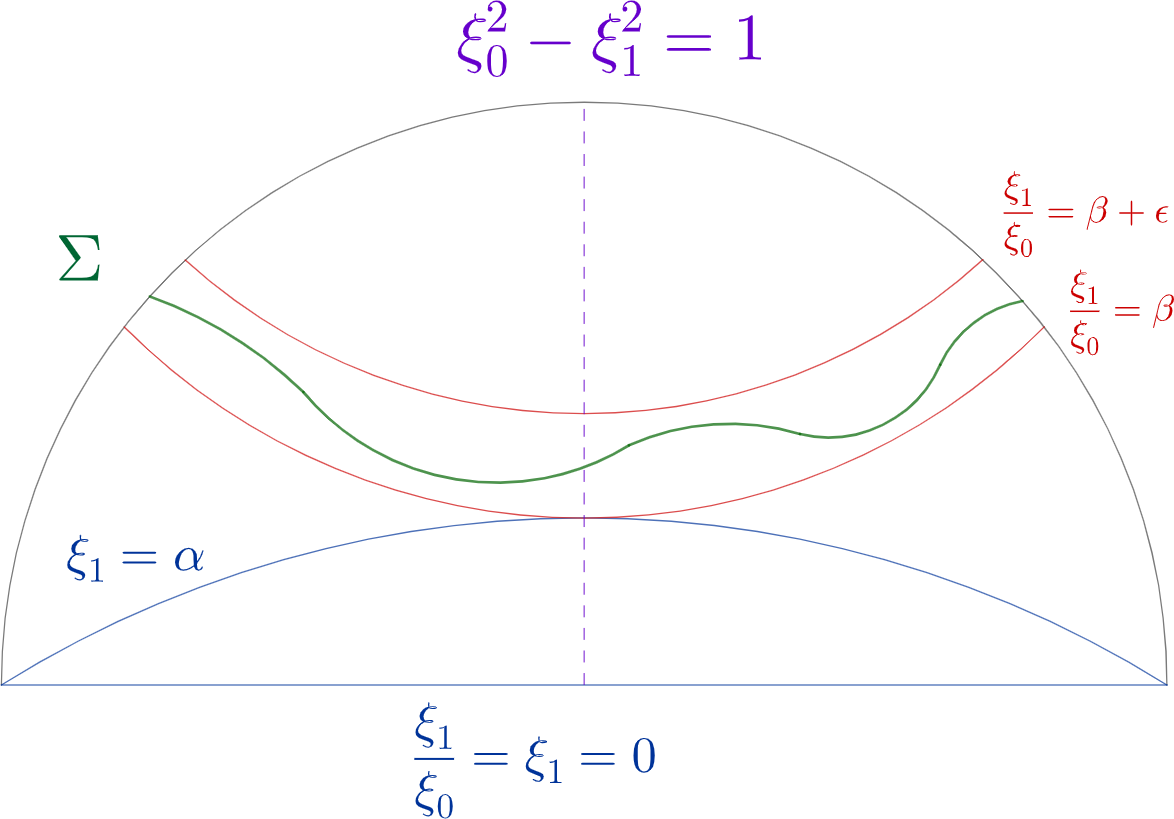
\includegraphics[width=6.5cm]{2021-04-28-space-est.png} 
    \caption{Level sets of \( y \) (totally geodesic, in red) and those of \( \xi_1 \) (in blue). The \( (n-1) \)-dimensional disks \( y=\beta\) and \( \xi_1 = \alpha = \frac{\beta}{\sqrt{1-\beta^2}} \) touch each other at the center.}
    \label{fig:space-est}
\end{figure}

\section{Weighted monotonicity in spaces with curvature bounded from above}
\label{sec:org2ac913f}
Fix a point \(O\) in a Riemannian manifold \((M^n,g)\), and let \(r_{\rm inj}\) be the
injectivity radius at \(O\). The Hessian of the distance function \(r\) to \(O\) is
given by:
\begin{equation}
\label{eq:hess-r}
\hess_p r (\partial_r, \cdot) =0, \qquad \hess_p r (v, v)=: I(v), \quad\forall p\in B(O,r_{\rm inj}),\ \forall v\perp \partial_r
\end{equation}
where \(I(v)=\int_{\Gamma}\left(|\dot V|^2 - K_M(\dot\gamma,V)|V|^2\right)\) is the index
form of the Jacobi field \(V\) along the geodesic \(\Gamma\) between \(O\) and \(p\) that
interpolates \(0\) at \(O\) and \(v\) at \(p\). 

When the sectional curvature
satisfies \(K_M\leq -a^2\) (respectively \(b^2\)), one can check that
\(I(v) \geq a\coth(ar)|v|^2\) (respectively \(b\cot (br)|v|^2\)). This gives an estimate of the \(\hess r\) on the
directions orthogonal to \(\partial_r\). By a change of variable, we can estimate the Hessian in a more isotropic way. 

\begin{proposition}[]
\label{prop:hess-r}
Inside \(B(O,r_{\rm inj})\), one has
\begin{enumerate}
\item \(\hess (a^{-2}\cosh ar) \geq \cosh ar.\ g\) if \(K_M\leq -a^2\).
\item \(\hess (-b^{-2}\cos br) \geq \cos br.\ g\) if \(K\leq b^2\) and \(r\leq \frac{\pi}{b}\).
\end{enumerate}
\end{proposition}
This means that the functions \(h=a^{-2}\cosh ar\) and \(h=-b^{-2}\cos br\) satisfy \(\hess h \geq
U.g\). 
We note that the functions \(U, V\) defined as in Proposition \ref{prop:cheeger-colding}
are still functions of \(h\): \(U= a^2 h\) (respectively \(-b^2 h\)) and \(V = |\nabla h|^2 = a^2
(h^2-1)\) (respectively \(-b^2 (h^2-1)\)) and one still has \(U = \frac{1}{2}V'\).

The \emph{eligible interval} \([0,r_{ \max})\) is defined to be \([0, r_{\rm inj})\) when
\(K_M\leq -a^2\) and \([0, \min (r_{\rm inj}, \frac{\pi}{2b}))\) when \(K_M\leq b^2\).

\begin{remark}
\label{rem:no-min-K}
\begin{enumerate}
\item When \(M\) is \(\mathbb{H}^n\) or \(\mathbb{S}^n\), the function \(h\) is the time-coordinate \(\xi_0\) and
the Euclidean coordinate \(x\) in Example \ref{ex:xi-H} and Example \ref{ex:xi-S}.
\item It follows from maximum principle and Proposition \ref{prop:hess-r} that there exists no closed
minimal surface in \(B(O, r_{\max})\). If \(M\) is Cartan--Hadamard (\(r_{\max}=+\infty\)) and if the boundary of a
minimal surface is contained in a geodesic ball, the entire surface stays inside that ball.
\end{enumerate}
\end{remark}

\subsection{Weighted monotonicity theorem}
\label{sec:orgb7c5ec5}

As explained in Remark \ref{rem:monotonicity-warped}, we can still have weighted
monotonicity theorem for the function \(h\). 
The \emph{weighted area} and \emph{weighted density} of a surface \(\Sigma^k\) are defined to be
\[
\bar A(\Sigma)(t):= \int_{\Sigma, r\leq t}U,\quad \bar\Theta(t):= \frac{\bar
A(\Sigma)(t)}{Q(t)}, \quad 
Q(t):= \begin{cases}
\frac{\omega_{k-1}}{k}\frac{\sinh^k at}{a^k}       ,  & \text{when } K_M\leq -a^2 \\
\frac{\omega_{k-1}}{k}\frac{\sin^k bt}{b^k}       , & \text{when } K_M\leq b^2
       \end{cases}
\]
Note that \(Q\) is the weighted area of a ball of radius \(t\) in the \(k\)-dimensional
space-forms of curvature \(-a^2\) or \(b^2\) and that the
density converges to 1 as \(t\) decreases to 0.


\begin{theorem}[]
\label{thm:monotonicity-geodesic}
Let \(M\) be a Riemannian manifold with sectional curvature \(K_M\leq -a^2\) or \(K_M\leq b^2\) 
and \(\Sigma^k\subset M\) be an extension of a minimal surface by geodesic cone, then
the density \(\bar\Theta(\Sigma)(t)\) is an increasing function in the eligible interval.
\end{theorem}

By a different argument than that of Corollary \ref{cor:sphere} and
Corollary \ref{cor:2pi}, one can prove that
the intersection curve of a minimal surface with a geodesic sphere of \(M\) is longer than the
great circle of the sphere of same radius in space-form.
\begin{corollary}[]
Let \(\Sigma^k\subset M\) be a minimal surface containing the point \(O\) with
multiplicity \(m\) and \(l_t
:= \vol_{k-1}\left(\Sigma\cap r^{-1}(t)\right)\). For all \(t\) in the eligible
interval, one has
\[
Q(t) \leq \bar A(\Sigma)(t)\leq \frac{l_t}{k}V(t)^{1/2}
\]
In particular, one has
\[
 l_t \geq \begin{cases}
 m\omega_{k-1}\left(\frac{\sinh at}{a}\right)^{k-1}	  ,  & \text{if $K_M\leq -a^2$} \\
 m\omega_{k-1}\left(\frac{\sin bt}{b}\right)^{k-1}	  , & \text{if $K_M\leq b^2$}
	  \end{cases}
\]
\end{corollary}
\begin{proof}
Instead of Lemma \ref{lem:less-than-tube} (see Remark \ref{rem:no-less-tube}), the upper estimate of \(\bar A\) follows from
\eqref{eq:stokes}:
\[
\bar A(\Sigma)(t) \leq \frac{1}{k}\int_{\Sigma, h=t}|\nabla^\Sigma h| \leq \frac{V(t)^{1/2}}{k}l_t.
\]
\end{proof}

\subsection{Comparison lemma}
\label{sec:orgffa9b3c}
It is more convenient see a weight \(P\) as a non-negative
continuous function of \(r\) instead of \(h\). The \emph{\(P\)-area} is defined as \(A_P(\Sigma)(t):= \int_{\Sigma, r\leq t}P(r)\) and the \emph{\(P\)-density} is \(\Theta_P:= \frac{A_P}{Q}\) where \(Q = Q_P\) is
\(P\)-area of a ball of radius \(r\) in space-form:
\begin{equation}
\label{eq:Q-geodesic}
 Q(t):= \begin{cases}
\omega_{k-1}\int_{r\leq t}P(r)\frac{\sinh^{k-1} ar}{a^{k-1}}dr       ,  & \text{when } K_M\leq -a^2 \\
\omega_{k-1}\int_{r\leq t}P(r)\frac{\sin^{k-1} br}{b^{k-1}}dr       , & \text{when } K_M\leq b^2
       \end{cases}
\end{equation}

\begin{lemma}[Comparison]
\label{lem:comparison-geodesic}
Let \(\Sigma^k\subset M\) be any surface not necessarily minimal and \(P_1,P_2\) be two
non-negative, continuous weight functions. Define \(Q_1, Q_2\) from \(P_1,
P_2\) as in \eqref{eq:Q-geodesic}. 
\begin{enumerate}
\item If \(P_1\) is weaker than \(P_2\), i.e. \(\frac{P_1}{Q_1} \leq
   \frac{P_2}{Q_2}\), and \(\frac{d}{dt}\Theta_2\geq 0\) in the eligible interval, then one has \(\Theta_1\leq\Theta_2\)
and
 \[
  \frac{d\Theta_1}{dt} \geq \frac{Q_2}{P_2}\frac{P_1}{Q_1} \frac{d\Theta_2}{dt}\geq 0
  \]
\item If \(P_2\) is weaker than \(P_1\) and \(\frac{d}{dt}\Theta_2\geq 0\) in the eligible interval, then one has \(\Theta_1\geq\Theta_2\)
\end{enumerate}
\end{lemma}

We note that it is necessary to mention \(a\) or \(b\) in order to compare two
weights. However, it can be checked that
\begin{lemma}[]
\label{lem:compare-geodesic}
For any \(a, b\geq 0\) and \(u\geq v \geq 0\),
\begin{enumerate}
\item \(P_1 = \cosh v r\) is weaker than \(P_2 = \cosh ur\) when \(K_M\leq -a^2\),
\item \(P_1 = \cos ur\) is weaker than \(P_2 = \cos vr\) in the interval \(t \leq \frac{\pi}{2u}\) when \(K_M\leq b^2\).
\end{enumerate}
\end{lemma}

\begin{remark}
\label{rem:compare-geodesic}
\begin{enumerate}
\item It follows from Lemma \ref{lem:compare-geodesic} and Theorem \ref{thm:monotonicity-geodesic} that for negatively curved space \(K_M\leq -a^2\), the monotonicity theorem holds for
any weight \(P_u =\cosh ur\) with \(u\in [0, a)\) and in particular the uniform weight
\(P_0 = 1\). One recovers the Theorem 1 of \cite{Anderson82_CompleteMinimalVarieties}.
\item When \(K_M\leq b^2\), the monotonicity theorem holds for any weight \(P_u = \cos
   ur\) with \(u\in[b,\infty)\) and the first part of Comparison Lemma 
could not be used on the uniform weight. However, one can still use the second part to
obtain  \(\Theta(t) \geq \bar\Theta(t) \geq  \text{multiplicity at $O$}\).
\end{enumerate}
\end{remark}

\begin{proposition}[]
\label{prop:uniform-area-sphere}
Suppose that \(K\leq b^2\), the minimal surface \(\Sigma^k\) contains a point \(O\) with multiplicity \(m\) and it has no boundary in the interior of \(B(O,t)\) for
certain \(t<r_{\max}\). Then
\[
A(\Sigma\cap B(O,t)) \geq m \omega_{k-1}\int_{r=0}^{t} \frac{\sin^{k-1}(br)}{b^{k-1}}dr
\]
In particular, if \(M\) is simply connected, with curvature pinched between \(\frac{b^2}{4}\) and \(b^2\) and \(\Sigma\subset M\) is a closed minimal surface, then
\begin{equation}
\label{eq:lower-area}
 A(\Sigma)\geq \frac{1}{2}\omega_k b^{-k}. 
\end{equation}
\end{proposition}

A weaker version of inequality \eqref{eq:lower-area}, with \(\frac{1}{2}\omega_k\) replaced by
the volume of the \emph{unit \(k\)-ball}, was proved in \cite{Hoffman.Spruck74_SobolevIsoperimetricInequalities}.

\begin{remark}
\label{rem:no-less-tube}
Lemma \ref{lem:less-than-tube} does not generalise because the \(P\)-area of a
geodesic cone in \(M\) is  no longer proportional to \(Q\).
\end{remark}

\begin{thebibliography}{EWW02}

\bibitem[AM10]{Alexakis.Mazzeo10_RenormalizedAreaProperly}
Spyridon Alexakis and Rafe Mazzeo.
\newblock Renormalized {Area} and {Properly} {Embedded} {Minimal} {Surfaces} in
  {Hyperbolic} 3-{Manifolds}.
\newblock {\em Commun. Math. Phys.}, 297(3):621--651, May 2010.

\bibitem[And82]{Anderson82_CompleteMinimalVarieties}
Michael~T. Anderson.
\newblock Complete minimal varieties in hyperbolic space.
\newblock {\em Inventiones Mathematicae}, 69(3):477--494, October 1982.

\bibitem[Ber21]{Bernstein21_SharpIsoperimetricProperty}
Jacob Bernstein.
\newblock A {Sharp} {Isoperimetric} {Property} of the {Renormalized} {Area} of
  a {Minimal} {Surface} in {Hyperbolic} {Space}.
\newblock {\em arXiv:2104.13317 [math-ph]}, April 2021.

\bibitem[CC96]{Cheeger.Colding96_LowerBoundsRicci}
Jeff Cheeger and Tobias~H. Colding.
\newblock Lower {Bounds} on {Ricci} {Curvature} and the {Almost} {Rigidity} of
  {Warped} {Products}.
\newblock {\em The Annals of Mathematics}, 144(1):189, July 1996.

\bibitem[CG92a]{Choe.Gulliver92_IsoperimetricInequalitiesMinimal}
Jaigyoung Choe and Robert Gulliver.
\newblock Isoperimetric inequalities on minimal submanifolds of space forms.
\newblock {\em Manuscripta Math}, 77(1):169--189, December 1992.

\bibitem[CG92b]{Choe.Gulliver92_SharpIsoperimetricInequality}
Jaigyoung Choe and Robert Gulliver.
\newblock The sharp isoperimetric inequality for minimal surfaces with radially
  connected boundary in hyperbolic space.
\newblock {\em Invent Math}, 109(1):495--503, December 1992.

\bibitem[CLY84]{Cheng.etal84_HeatEquationsMinimal}
Shiu-Yuen Cheng, Peter Li, and Shing-Tung Yau.
\newblock Heat {Equations} on {Minimal} {Submanifolds} and {Their}
  {Applications}.
\newblock {\em American Journal of Mathematics}, 106(5):1033, October 1984.

\bibitem[EWW02]{Ekholm.etal02_EmbeddednessMinimalSurfaces}
Tobias Ekholm, Brian White, and Daniel Wienholtz.
\newblock Embeddedness of {Minimal} {Surfaces} with {Total} {Boundary}
  {Curvature} at {Most} \$4{\textbackslash}pi\$.
\newblock {\em Annals of Mathematics}, 155(1):209--234, 2002.

\bibitem[GW99]{Graham.Witten99_ConformalAnomalySubmanifold}
C.~Robin Graham and Edward Witten.
\newblock Conformal {Anomaly} {Of} {Submanifold} {Observables} {In} {AdS}/{CFT}
  {Correspondence}.
\newblock {\em Nuclear Physics B}, 546(1-2):52--64, April 1999.
\newblock arXiv: hep-th/9901021.

\bibitem[HS74]{Hoffman.Spruck74_SobolevIsoperimetricInequalities}
David Hoffman and Joel Spruck.
\newblock Sobolev and isoperimetric inequalities for riemannian submanifolds.
\newblock {\em Comm. Pure Appl. Math.}, 27(6):715--727, 1974.

\bibitem[Law70]{Lawson70_GlobalBehaviorMinimal}
H.~Blaine Lawson.
\newblock The {Global} {Behavior} of {Minimal} {Surfaces} in
  \${S}{\textasciicircum}n\$.
\newblock {\em The Annals of Mathematics}, 92(2):224, September 1970.

\bibitem[Mor16]{Morgan16_GeometricMeasureTheory}
Frank Morgan.
\newblock {\em Geometric measure theory: a beginner's guide}.
\newblock Elsevier/AP, Amsterdam ; Boston, 2016.

\bibitem[Sch21]{Scharrer21_GeometricInequalitiesVarifolds}
Christian Scharrer.
\newblock Some geometric inequalities for varifolds on {Riemannian} manifolds
  based on monotonicity identities.
\newblock {\em arXiv:2105.13211 [math]}, May 2021.
\newblock arXiv: 2105.13211.

\end{thebibliography}

\end{document}

%%% Local Variables:
%%% mode: latex
%%% TeX-master: t
%%% End:
